\chapter{Technical Design}

This chapter describes the design and choices behind the technological systems which lay the foundation for the application. The development environment is based around Unreal Engine and \cpp.

\section{System Architecture}

The code architecture is based around the object-oriented nature of \cpp and patterns within game programming. Limited by the development environment, we had to implement all classes as derivatives from Unreal Engine's base classes. These classes enable common functionality such as rendering, collisions and mathematical operations such as translation and rotation. We continued this style of inheritance, defining base properties for objects, and deriving further into special classes if needed. A prime example of this is in the editor mode of the application, where each object in a level is treated as an \textit{EditorObject}, including trains and railways. An \textit{EditorObject} is an interactable entity in a level. These can be manipulated by the \textit{EditorController}, which handles all user input and level manipulation.

\section{Application module Architecture}
The application's hierarchy has been divided into four figures for clarity. The model's shows all the actors, pawns, widgets, etc, and tries to visualize their inter-connectivity in the system.

Figure \ref{LoginHierFigure} shows the different game modes a level can open as and what HUD is used for the game modes. Both game mode and HUD will be explained in more detail in \ref{implementation_chapter} and \ref{HUD_implementation} respectively.

\begin{figure}[H]
    \centerline{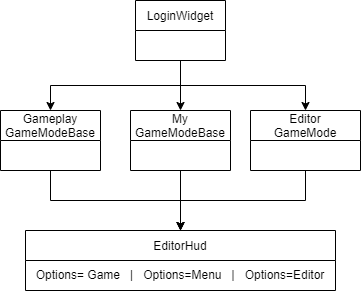
\includegraphics[width=0.6\textwidth]{figures/Untitled Diagram-Login.drawio.png}}
    \caption[Hierarchy of application start up functionality ]{ }
    \label{LoginHierFigure}
\end{figure} 

To decide what HUD elements should be displayed, an Options string is sent with the new game mode. This string could either be blank, which defaults to Menu, "Game" to start a level in simulating mode or "Editor" to start the level in editor mode. The three next figures displays the hierarchy of these three gamemodes respectively.
\begin{figure}[H]
    \centerline{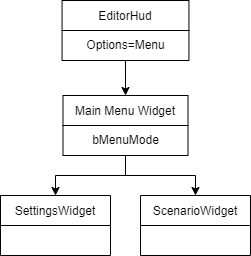
\includegraphics[width=0.5\textwidth]{figures/Untitled Diagram-Main Menu.drawio.png}}
    \caption[Hierarchy of application start up functionality ]{The module hierarchy for main menu mode }
    \label{fig::menu_hierarcy}
\end{figure} 

\begin{figure}[H]
\centering
\begin{minipage}{.5\textwidth}
  \centering
  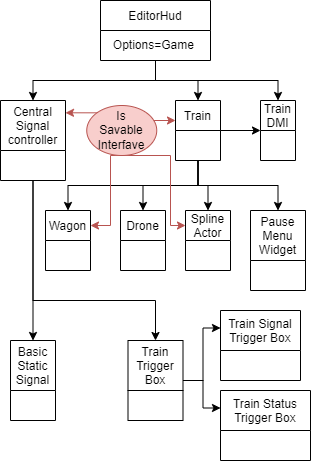
\includegraphics[width=0.95\linewidth]{figures/Untitled Diagram-Game.drawio.png}
  \captionof{figure}{The module hierarchy for simulating mode}
  \label{fig:sim_mode}
\end{minipage}%
\begin{minipage}{.5\textwidth}
  \centering
  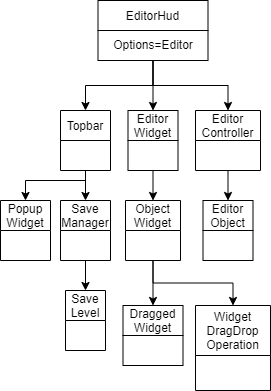
\includegraphics[width=0.95\linewidth]{figures/Untitled Diagram-Editor.drawio.png}
  \captionof{figure}{The module hierarchy for editor mode}
  \label{fig:editor_mode}
\end{minipage}
\end{figure}





\section{Network Architecture}

Authentication is currently the only system which uses the network. While multiplayer is a feature used in the existing \gls{desksim} solution, it is not a part of this demo. 

User authentication is done using the existing solution in use at Lokførerskolen. Their system uses two endpoints, the first receives a username and password and returns a JWT (JSON Web Token) on success. The JWT is then sent to the second endpoint, which returns a JSON UserObject which contains info such as ID, Username, Roles, etc. 

When the program is launched a login screen is presented to the user, where a username and password must be entered. The user must be authenticated in order to use the software. If an error such as invalid username or password, or an error with the server occurs, an error message is shown to the user. Once the user is authenticated their info is stored for the duration of the session. The user-info is never stored to any file, which means the user needs to log in each time the program is started. Because the username, password nor token is ever stored locally, they cannot be extracted from local files in order to obtain private credentials.


%\vspace*{1 cm} %Temporary fix for tables going into eachother
\begin{figure}[H]
    \centerline{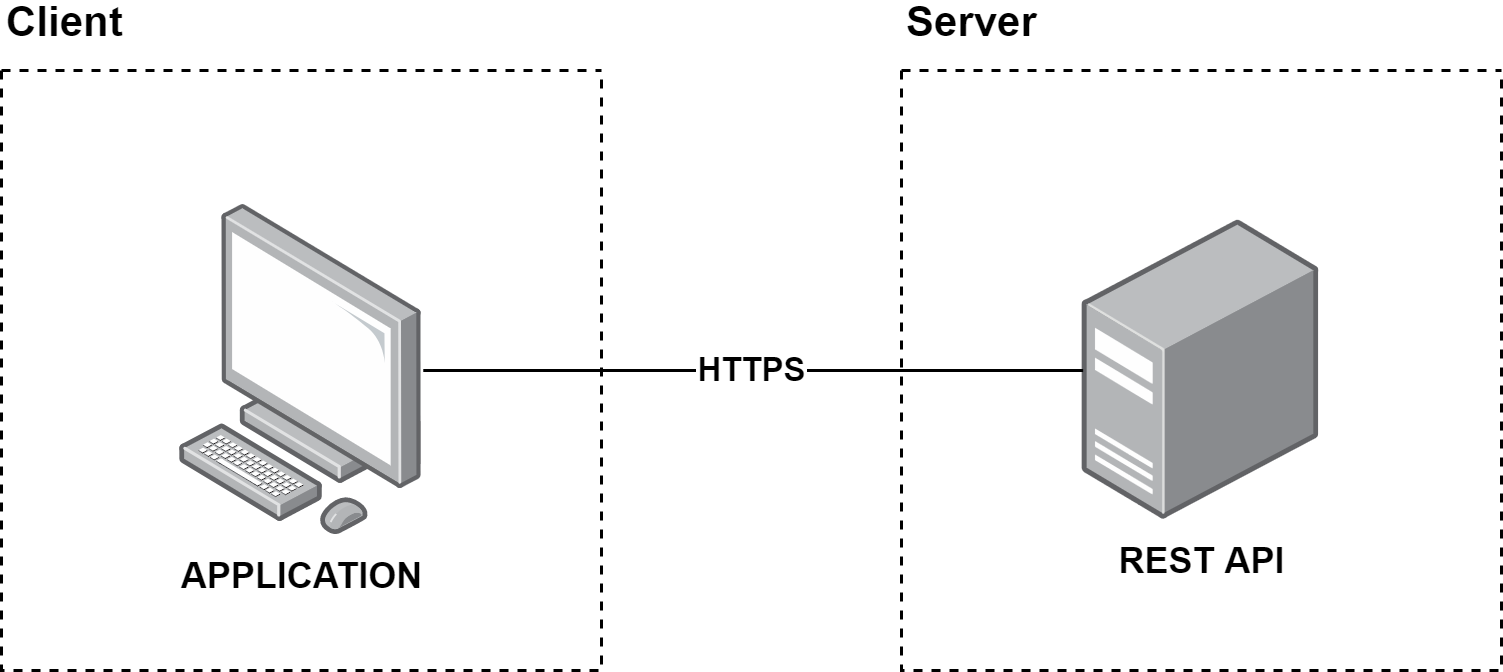
\includegraphics[width=0.9\textwidth]{figures/NetworkArchitecture.png}}
    \caption{A diagram for the network architecture}
\end{figure} 

\subsection{File Structure}
Unreal Engine separates files into two main folders, \verb|Source| for code files and \verb|Content| for asset files. We decided to structure the code files into folders based on their area of use in the context of the software. All other asset files were separated based on their type inside the \verb|Content|-folder.


\begin{figure}[h]
    \centering
    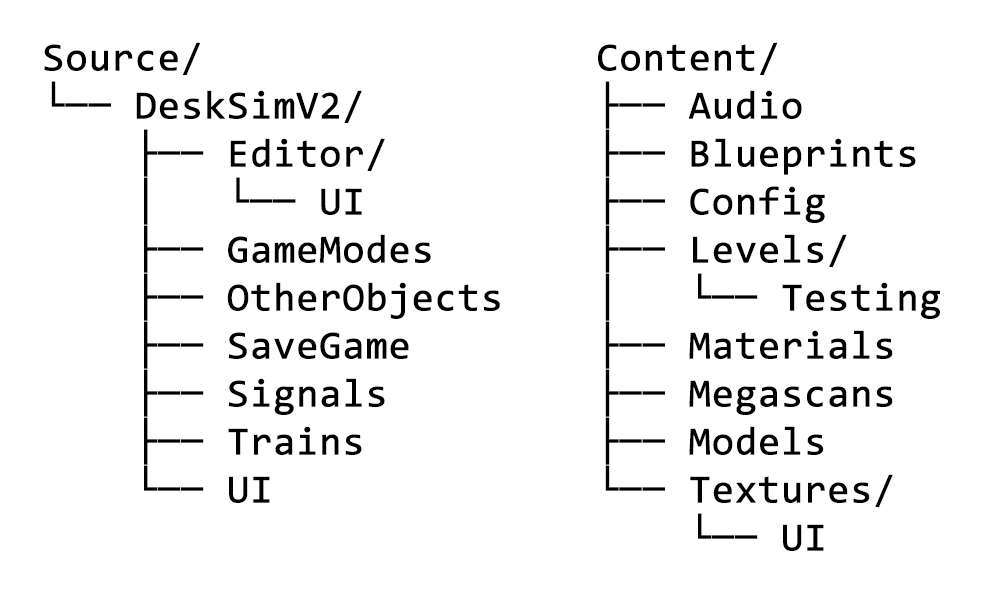
\includegraphics[width=0.75\textwidth]{figures/Files3.png}
    %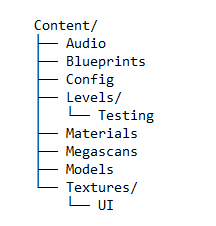
\includegraphics[width=0.4\textwidth]{figures/Files2.png}
    %\vspace{-12pt}
    \caption{File hierarchy for Source and Content}
    \label{Stop_Signal_img}
\end{figure} 


%\subsubsection{Scenarios}
% System
%\subsection{Design choices}
% 

% Have to figure out what to include in this section!
